\documentclass[a4paper,12pt]{article} % тип документа

% Поля страниц
\usepackage[left=2.5cm,right=2.5cm, top=2cm,bottom=2cm,bindingoffset=0cm]{geometry}
    
%Пакет дял таблиц   
\usepackage{multirow} 
    
%Отступ после заголовка    
\usepackage{indentfirst}


% Рисунки
\usepackage{subcaption,floatrow,graphicx,calc}
\usepackage{wrapfig}

% Создаёем новый разделитель
\DeclareFloatSeparators{mysep}{\hspace{1cm}}

% Ссылки?
\usepackage{hyperref}
\usepackage[rgb]{xcolor}
\hypersetup{				% Гиперссылки
    colorlinks=true,       	% false: ссылки в рамках
	urlcolor=blue          % на URL
}


%  Русский язык
\usepackage[T2A]{fontenc}			% кодировка
\usepackage[utf8]{inputenc}			% кодировка исходного текста
\usepackage[english,russian]{babel}	% локализация и переносы


% Математика
\usepackage{amsmath,amsfonts,amssymb,amsthm,mathtools, mathrsfs, wasysym}


\begin{document}
\begin{center}
	\footnotesize{ФЕДЕРАЛЬНОЕ ГОСУДАРСТВЕННОЕ АВТОНОМНОЕ ОБРАЗОВАТЕЛЬНОЕ 			УЧРЕЖДЕНИЕ ВЫСШЕГО ОБРАЗОВАНИЯ}\\
	\footnotesize{МОСКОВСКИЙ ФИЗИКО-ТЕХНИЧЕСКИЙ ИНСТИТУТ\\(НАЦИОНАЛЬНЫЙ 			ИССЛЕДОВАТЕЛЬСКИЙ УНИВЕРСИТЕТ)}\\
	\footnotesize{ФАКУЛЬТЕТ ОБЩЕЙ И ПРИКЛАДНОЙ ФИЗИКИ\\}
	\hfill \break
	\hfill\break
	\hfill\break
	\hfill \break
	\hfill \break
	\hfill \break
	\hfill \break
	\hfill \break
	\hfill \break
	\hfill \break
	\hfill \break
	\hfill \break
	\hfill \break
	\hfill \break
	\large{Лабораторная работа № 4.4.1 \\\textbf{Амплитудная дифракционная решетка}}\\
	\hfill \break
	\hfill \break
	\hfill \break
	\begin{flushright}
		Серебренников Даниил\\
		Группа Б02-826
	\end{flushright}
	\hfill \break
	\hfill \break
	\hfill \break
	\hfill \break
	\hfill \break
	\hfill \break
	\hfill \break
	\hfill \break
	\hfill \break
	\hfill \break
	\hfill \break
\end{center}
\begin{center}
	Долгопрудный, 2020 г.
\end{center}
\thispagestyle{empty}
\newpage
	\textbf{Цель работы:} знакомство с работой и настройкой гониометра Г5, определение спектральных характеристик амплитудной решетки.

	\textbf{В работе используются:}  гониометр, дифракционная решетка, ртутная лампа.
\section{Теоретическая часть}
	\noindent Основное соотношение приближенной теории дифракционной решётки:
	\begin{equation}
	d\sin \varphi_m = m\lambda.
	\end{equation}
	Угловая дисперсия $D$ характеризует угловое расстояние между близкими спектральными линиями:
	\begin{equation}
	D = \frac{d\varphi}{d\lambda} = \frac{m}{d \cos \varphi}=\frac{m}{\sqrt{d^{2}-m^{2} \lambda^{2}}}.
	\end{equation}
	
\section{Экспериментальная установка}
	При работе с дифракционной решёткой основной задачей является точное измерение углов, при которых наблюдаются главные максимумы для различных длин волн. В нашей работе для измерения углов используется гониометр Г5. Принципиальная схема экспериментальной установки приведена на рис. \ref{inst}.
	\begin{figure}[H]
		\caption{Схема установки.}
		\label{inst}
		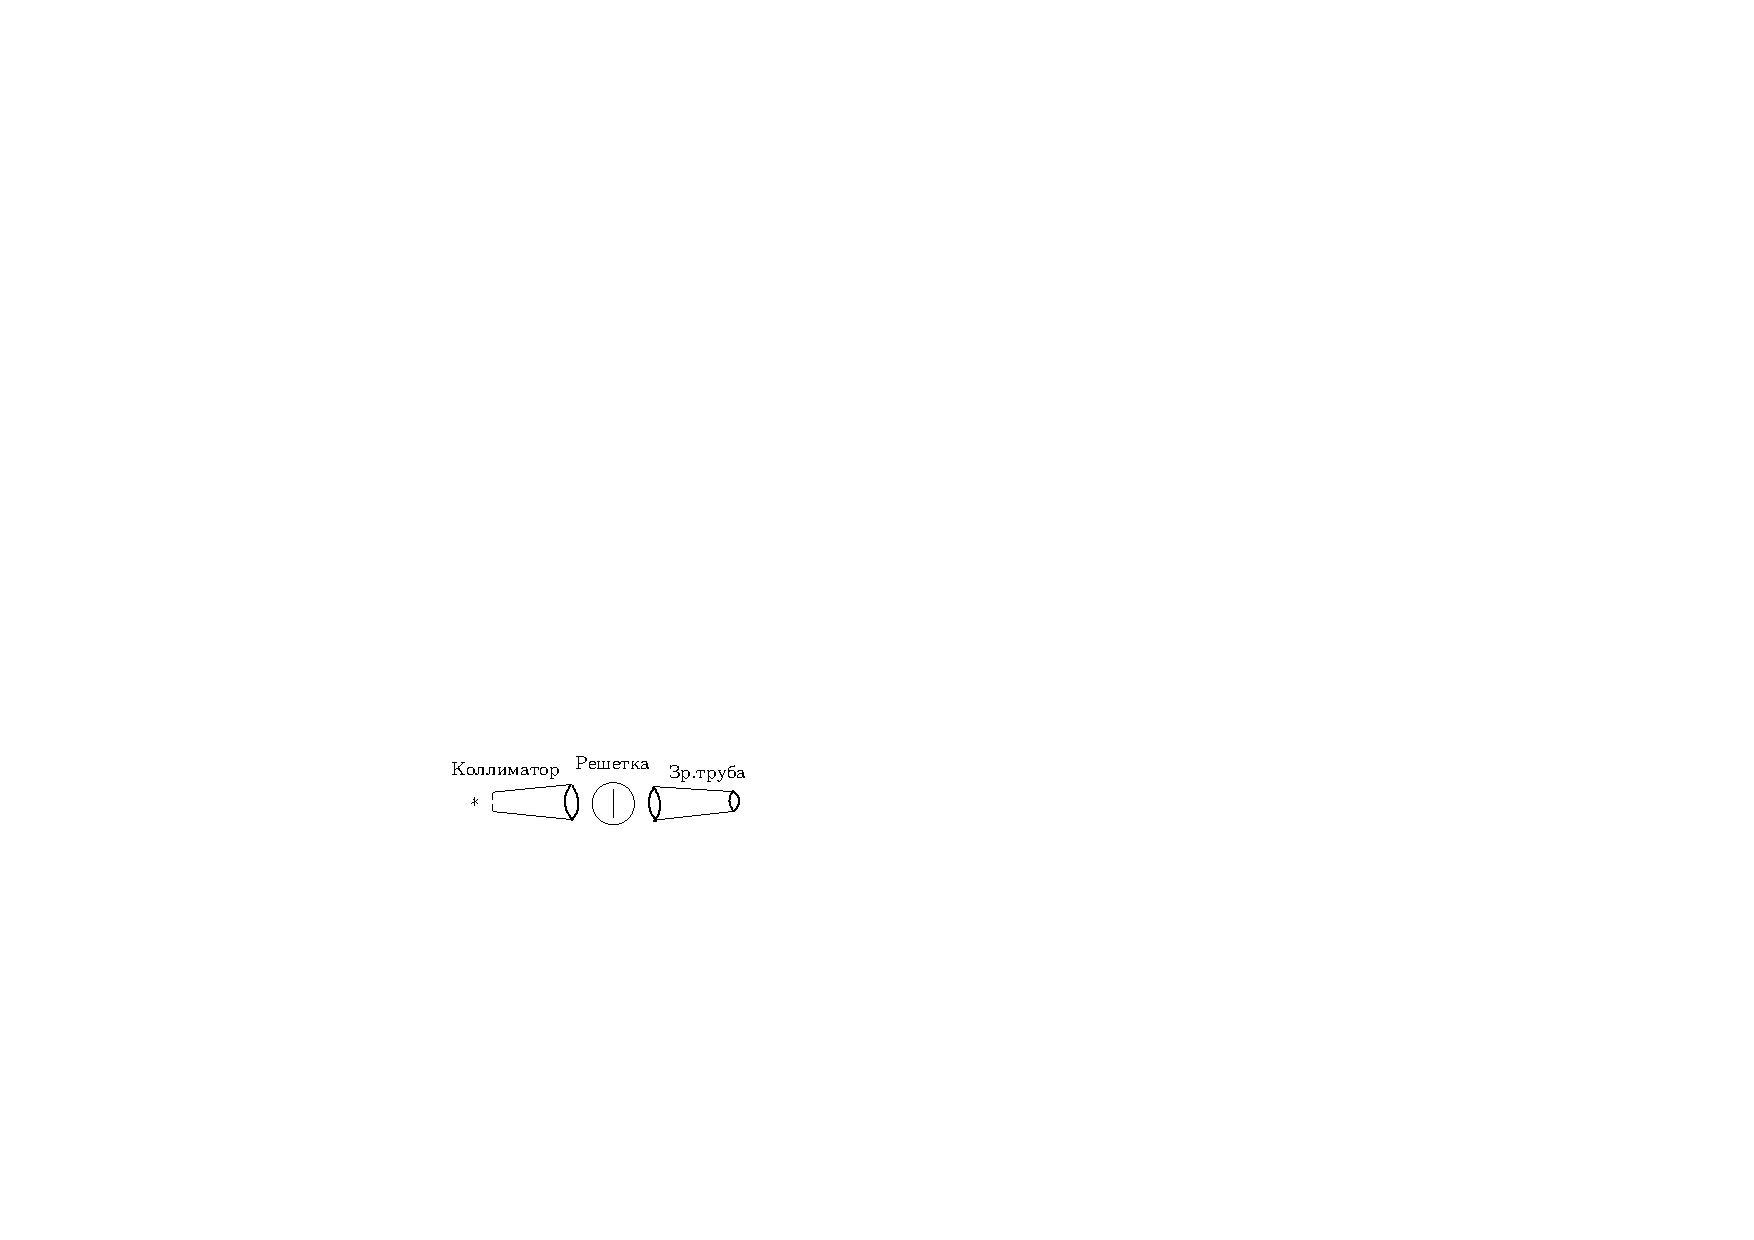
\includegraphics[scale=1.5]{inst.pdf}
	\end{figure}

\newpage
\section{Экспериментальная часть}
	\subsection{Экспериментальные данные}
		Измерим угловые координаты спектральных линий ртути в $ \pm1 $ порядках, рассчитаем углы дифракции $\varphi_m$. Результаты измерений и вычислений занесем в таблицу~\ref{table:exp1}.
		\floatsetup[table]{capposition=top}	
		\begin{table}[H]
			\caption{}
			\label{table:exp1}
			\begin{tabular}{|p{0.96cm}|p{2.2cm}|p{1.5cm}|p{1.5cm}|p{1.5cm}|p{1.5cm}|p{1.5cm}|p{1.5cm}|p{1.5cm}|}
				\hline
				& фиолетовый & синий  & голубой & зеленый & желтый & желтый & красный & красный \\ \hline
				$ \varphi $& $11^{\circ}40'56''$ & $12^{\circ}33'27'' $& $14^{\circ}12'11''$ & $15^{\circ}49'12'' $& $16^{\circ}47'22'' $& $16^{\circ}48'12''$ & $17^{\circ}48'15'' $& $18^{\circ}08'15''$ \\ \hline
				$\sin \varphi$& 0,2022     & 0,2171 & 0,2451  & 0,2723  & 0,2886 & 0,2888 & 0,3055  & 0,3110  \\ \hline
				$ \lambda $, нм & 404,7      & 435,8  & 491,6   & 546,1   & 577    & 579,1  & 623,4   & 690,7   \\ \hline
			\end{tabular}
		\end{table}
		Для оценки угловой дисперсии решётки определим разности угловых координат линий жёлтого дублета во всех видимых порядках ($ \Delta \lambda = 21  \buildrel _{\circ} \over {\mathrm{A}} $):
		\floatsetup[table]{capposition=top}	
		\begin{table}[H]
			\caption{}
			\label{table:exp2}
			\begin{tabular}{|r|c|c|c|}
				\hline
				$m$  & $ \Delta \varphi , ''$  & $D$ exp,  $ 10^{-5} $ рад/$  \buildrel _{\circ} \over {\mathrm{A}}$   & $D$ teor,   $ 10^{-5} $ рад/$  \buildrel _{\circ} \over {\mathrm{A}}$   \\ \hline
				1  &50      & $1,14\pm 0,16$ & $5,22$  \\ \hline
				-1 & 239     &$-5,46\pm0,16$ & $-5,22$ \\ \hline
				2  & 588     &$13,4\pm0,1$ & $12,2$  \\ \hline
				-2 & 548     &$-12,5\pm 0,1$ & $-12,2$ \\ \hline
				3  & 	1350    &$30,9\pm 0,1$ & $29,9$  \\ \hline
				-3 &1332    & $-30,4\pm 0,1$ & $-29,9$ \\ \hline
			\end{tabular}
		\end{table}

	\subsection{Обработка результатов}
		Построим график зависимости $\sin \varphi_m$ от длины волны $\lambda$ для $\pm 1$ порядка:
		\begin{figure}[h!]
			\begin{floatrow}
				\ffigbox[\FBwidth]{\caption{Зависимость $\lambda$ от $\sin \varphi_m$.}\label{fig:Graph_1}}%
				{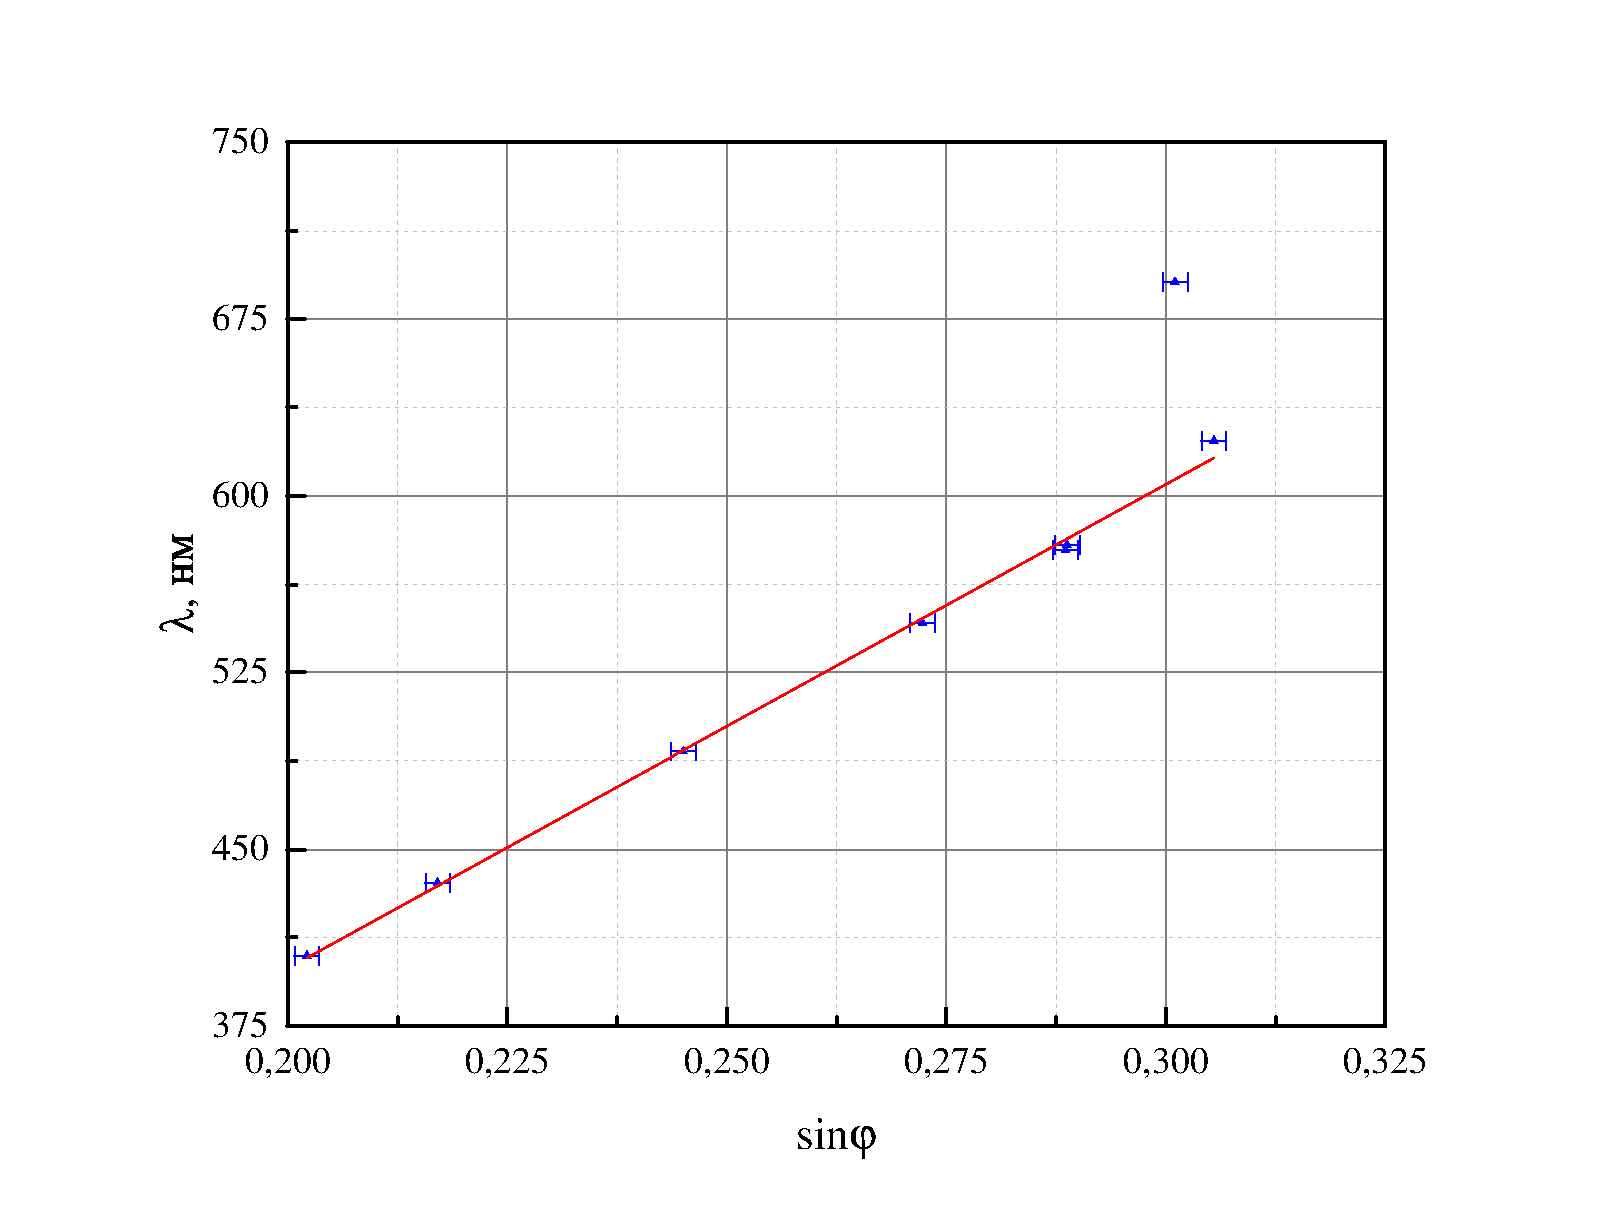
\includegraphics[width=8cm,height=7cm]{graph1}}    
			\end{floatrow}
		\end{figure}
	
		Определим по углу наклона графика период решётки $d$:
		\begin{equation}
			d = (2,1\pm 0,2) \ \text{мкм}.
		\end{equation}
	
		Оценим разрешимый спектральный интервал $ \delta\lambda $, разрешающую способность $ R $ и число эффективно работающих штрихов решётки $ N $, а также её эффективный размер $ l $:
		\begin{equation}
			\delta\lambda \approx \Delta\varphi/D = 2 \buildrel _{\circ} \over {\mathrm{A}};
		\end{equation}
		\begin{equation}
			R \approx \frac{\lambda}{\delta\lambda} = 2885
		\end{equation}
		\begin{equation}
			N \approx R/m = 2885
		\end{equation}
		\begin{equation}
			l \approx Nd = 6\; \text{мм.}
		\end{equation}
		
\section{Выводы}
	Таким образом, мы исследовали спектральные линии ртути, определили шаг решётки, её угловую дисперсию, а также её эффективный размер. Полученные результаты близки к теоретическим вычислениям, за исключением первого порядка; возможно, это связано с неправильным измерением.



































\end{document}